\section{System Model And Assumptions}
\label{sec:assumptions}

{\bf Power Management Architecture.} Figure~\ref{fig:SmartGridArchi-fig} shows
the architecture of a future generation smart grid (SmartGrid)~\cite{huang11}.
The system is essentially a microgrid consisting of energy storage devices
(DESD), energy resources (DRER) and LOADs. Each node is potentially owned and
located in a residence or business and the basic idea is to share power among
nodes in order to benefit the overall system. Intelligent flow controllers
(nodes) contain Solid State Transformers (SSTs), that are physical actuators
controlling power flow to and from a shared electrical bus under the direction
of co-operating Distributed Grid Intelligence (DGI) processes.

The DGI processes are cyber algorithms that choose, negotiate and manage power
transfers among nodes based on local information and information about the
states of other nodes that is periodically exchanged among nodes. In the current
work, we assume that all nodes are synchronized, for the sake of simplicity.
Nodes periodically exchange state information with each other in a state
collection phase. Next, a negotiation phase is performed in which nodes conduct
negotiations to identify which power transfers need to be performed among nodes.
The identified power transfers between pairs of nodes are then performed in a
power transfer phase. One cycle is depicted in Figure\ref{fig:cycle}, with one
or more negotiation and power transfer phase pairs after a state collection
phase. This entire cycle of state collection, negotiation and power transfer
phases is repeated.

\begin{figure}[htb]
  \begin{center}
    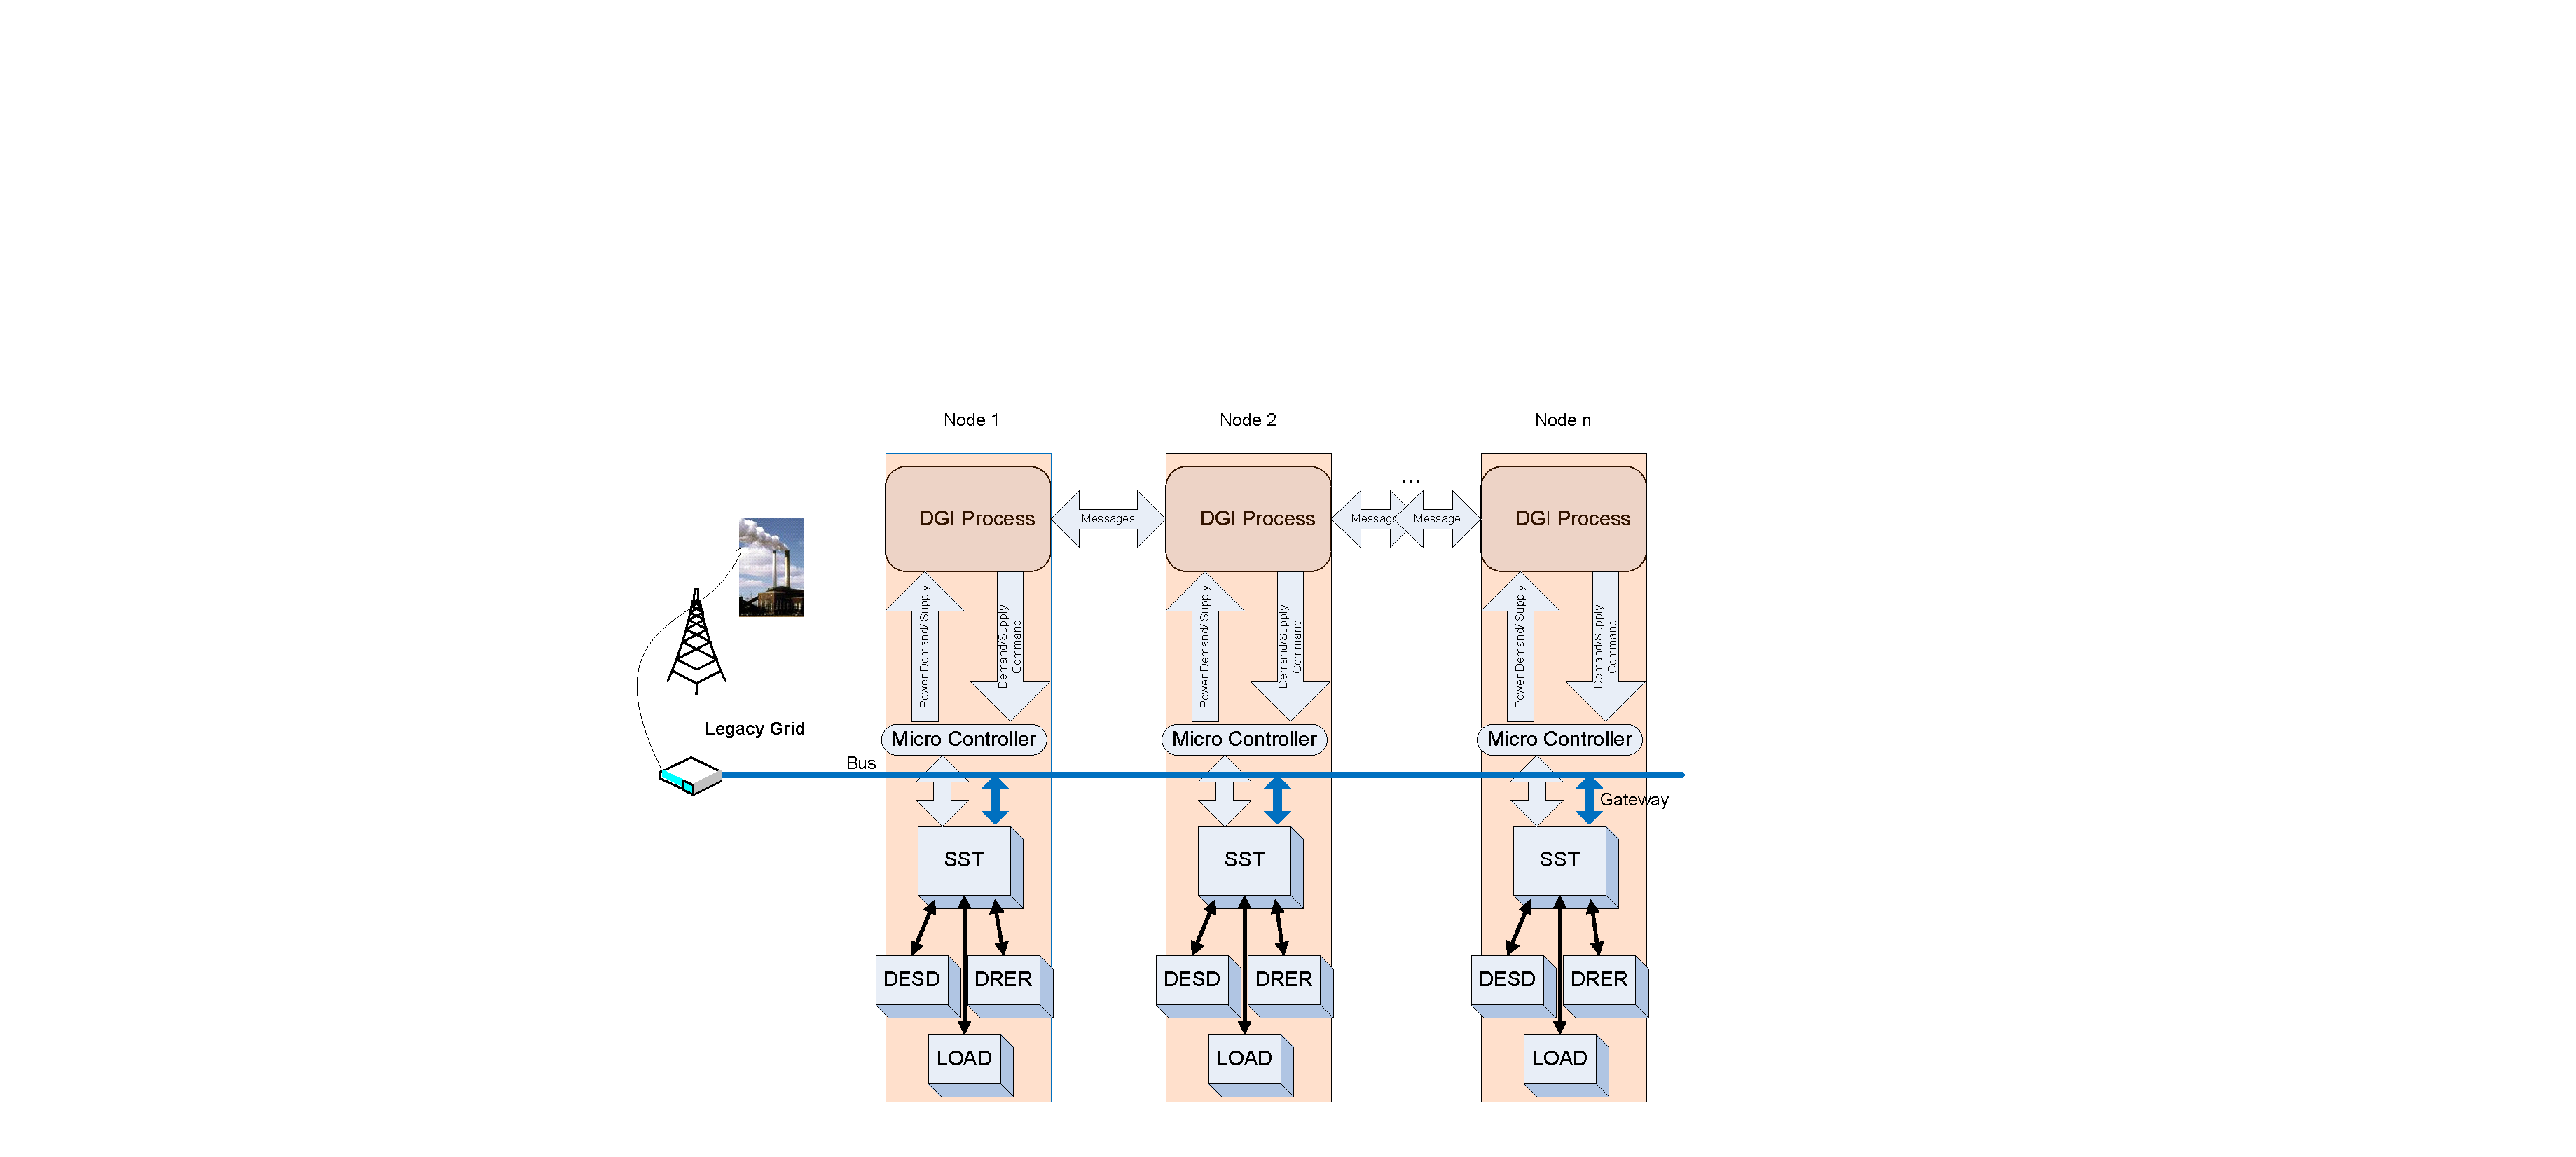
\includegraphics[width=0.45\textwidth]{Figures/DistributedLoadBalancing3.pdf}
  \caption{Smart Grid Power Management Architecture}
  \label{fig:SmartGridArchi-fig}
  \end{center}
\end{figure}

\begin{figure}[htb]
  \begin{center}
    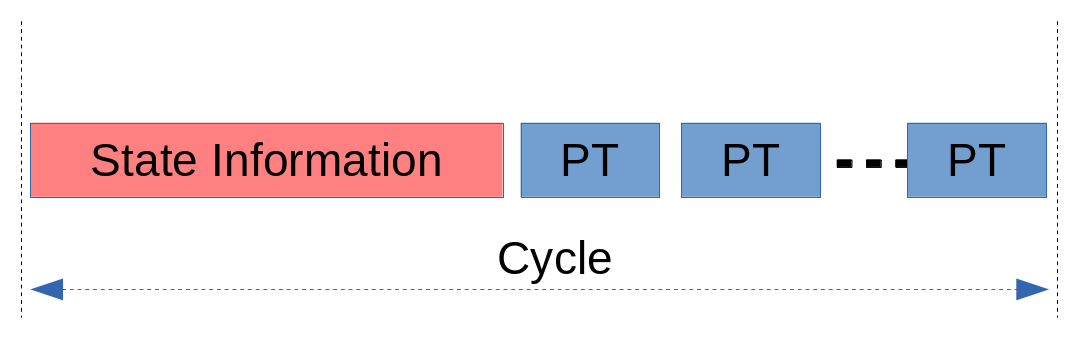
\includegraphics[width=0.45\textwidth]{Figures/cycle_fig.png}
  \caption{A single cycle of collecting state information followed by many negotiation and power transfer phases (PT)}
  \label{fig:cycle}
  \end{center}
\end{figure}

{\bf Power Transfer Model.} Power transfers within one phase are performed as a
series of (periodic) power migrations, each transferring a given quantum (say
$\delta$) of power. The cyber algorithm on the source (sender) node sends
appropriate control signals to the local physical actuators to add a quantum of
power to the electrical bus and sends a power migration message to the
destination (receiver) node signaling this. Upon receiving this power migration
message, the destination node sends control signals to its local physical
actuators to remove a quantum of power from the electrical bus and sends an
acknowledgement message to the source node.

{\bf Physical System Model.} The physical system is a finite inertia microgrid,
that is, a power system with a small number of generators and loads that acts
independently of the grid. There is a relatively small rotating generator,
whose inertia dominates the dynamics as described in the next section. There
are some number of controllable nodes that participate in the power management
by acting as either loads or generators. Nodes with excess generating capacity
transfer power to nodes that have excess load.

{\bf Communication Model.} 
Each node in the network runs an adaptive message scheduling algorithm that schedules power migrate messages in any given 
topology, based on the observed communication latencies at a given node. 
